\section{Receiver EPS}
\label{receiver_EPS}

De EPS system of the receiver is almost the same as that of the emitter.

The required power generation is 42W, resulting in a required area of 0.5 square meters. Again the STK program was used to verify that the assumed cosine loss value was correct. The calculated power generation for 0.5 square meters was 52.5W, thus again it is shown that the value was correct.

Because the power requirement is much less also the amount of batteries necessary was less. For the receiver, only one battery with 2 modules was needed to be able to power the satellite during eclipse.
\\\\

\begin{table}[H!]
\centering
\begin{tabular}{cccccc}
\toprule
Part & \multicolumn{3}{c}{Dimensions [mm]} & Weight [g] & Power usage [W]\\ 
\midrule
 & Length & Width & Height & & \\ 
 Driver (2 needed) & 30 & 6 & 60 & 21.4 & 1 \\ 
 SMA Deployment  (2 needed) & 120 & 50 & 10 & 120 & 4* \\ 
 Battery & 168 & 102 & 10 & 1000 & 0 \\ 
 Convertor & 95 & 60 & 17 & 80 & 1.5 \\ 
 Shunt regulator  (2 needed) & 2.8 & 2.6 & 1.05 & 0.1 & 0.5 \\ 
 Thermal knife (2 needed) & 60 & 50 & 38 & 280 & 15**  \\
 Wiring & - & - & - & 230 & 0.28 \\ 
 Solar panels (2 needed) & 500 & 500 & 0.75 & 1.2 & 0 \\
 \midrule
 TOTAL & - & - & - & 2593.5 & 4.875***  \\ 
\bottomrule
 \multicolumn{6}{l}{* for 4 minutes} \\
 \multicolumn{6}{l}{** for 60 seconds} \\
 \multicolumn{6}{l}{*** continuous power usage only} \\
\end{tabular}
\caption{EPS subpart details for receiver satellites}
\label{tab:EPS_details}
\end{table}


As with the emitter, here the architecture of the power system of the receiver is show in figure \ref{fig:receiver_block}. The power from the solar panels is transferred to the dc-dc convertor. There part of it is sent to charge the batteries and part is sent to power the payload. During eclipse periods, the power is sent from the batteries to the payload via the convertor.

\begin{figure}[H!]
\centering
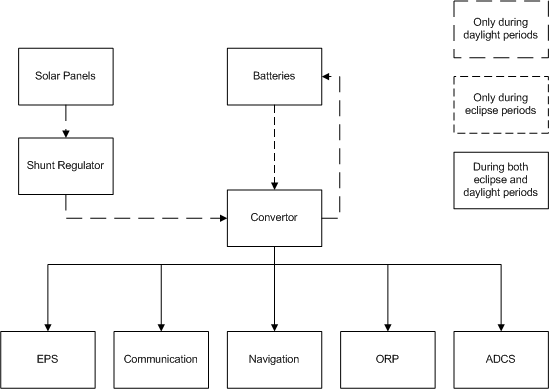
\includegraphics{img/EPS receiver block diagram.png}
\caption{Electrical block diagram of the receiver}
\label{fig:receiver_block}
\end{figure}